\chapter{Enhanced ASR}
\label{chap:enhanced_asr}

\iffalse
\begin{figure}[hb!]
	\centering
	\resizebox{.9\textwidth}{!}{
		\begin{tikzpicture}[thick, node distance=4.5cm, 
		>=stealth,
		bend angle=45,
		auto]
		\draw
		node at (0,0)[draw,trapezium,trapezium left angle=70,trapezium right angle=-70] (sound) {sound}
		node [block, right=1.5cm of sound] (acm) {\shortstack{Acoustic model\\ \tiny{Jasper}}}
		node [block, below= 1.5cm of acm] (cor) {\shortstack{Translation model\\ \tiny{Transformer}}}
		node [draw,trapezium,trapezium left angle=70,trapezium right angle=-70, right =1.5cm of cor] (trans) {\shortstack{transcript\\ \tiny{graphemes}}};
		
		\draw[->](sound) -> node {}  (acm);
		\draw[->](acm) -> node  {phonemes} (cor);
		\draw[<-](trans) -> node {}  (cor);
		
		\end{tikzpicture}}
	\caption{Enhanced ASR pipeline. The input sound is first transcribed to phonemes using Jasper/QuartzNet ``acoustic'' model. Phonemes are fed to the ``translation'' model. Translation model not only translates, but also fixes some errors in the ASR output and produces orthographic transcriptions.}
	\label{fig:asr_enhanced_pipeline_}
\end{figure} 
\fi

\begin{figure}[t]
	\centering
	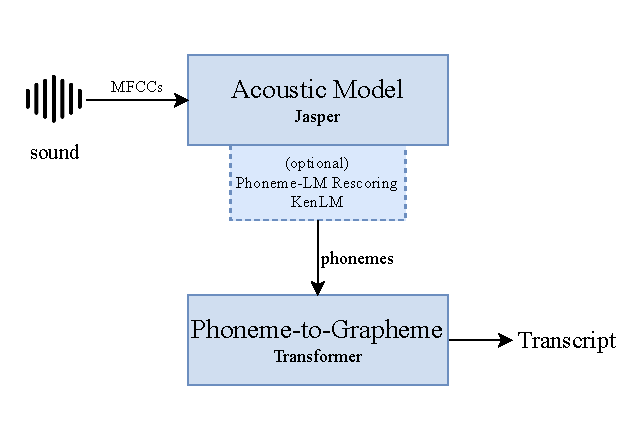
\includegraphics[width=.9\textwidth]{img/easr2}
	\caption{Enhanced ASR pipeline. The input sound is first transcribed to phonemes using Jasper/QuartzNet ``acoustic'' model. Phonemes are fed to the ``translation'' model. Translation model not only translates, but also fixes some errors in the ASR output and produces orthographic transcriptions.}
	\label{fig:asr_enhanced_pipeline}
\end{figure} 


In this chapter, we describe and build enhanced ASR. We propose to split a conventional end-to-end ASR into to two successive models: 

\begin{enumerate}
	\item an ``acoustic'' model that outputs phonemes instead of graphemes,
	\item a ``translation'' model that consumes the phonemes and translates them to the graphemes.
\end{enumerate}

An illustration of the proposed enhanced ASR pipeline is in \cref{fig:asr_enhanced_pipeline}.

The added hope is that the translation model right after the ``acoustic'' model will not only ``blindly'' translate phonemes into graphemes, but also correct errors. Errors can occur, for example, due to adverse conditions during voice recording (e.g., background noise), speaker's dialect, or pronunciation errors. Some of these errors may be obscure for a person, as we are naturally able to communicate in a noisy environment. The motivation for the introduction of such a translation step into our pipeline is that such a model better ``understands the language'' and can take an extended context into account compared to the rather convolutional Jasper model. Furthermore, we can utilize other non-speech corpora, e.g., available monolingual data to train this part of our pipeline.

We decided to use phonemes as an intermediate representation. We believe that conventional grapheme representation is too complicated and constrained for some languages with complicated rules of mapping speech to a transcript. This issue becomes immense when dealing with dialects and non-native speakers. The translation model in the second step thus may be a better fit for this transformation.

Step by step, we describe the selection of hyperparameters and training of the translation model for the enhanced ASR pipeline. First, we discuss and experiment with source encoding, and afterwards, we train the model.

The chapter is organized as follows: we first review related work in \cref{easr:related}. In \cref{easr:tokenizer}, we experiment with various approaches to text encoding. In \cref{easr:english} we present the main objective of this chapter --- translation model for ASR.





\section{Related Work}
\label{easr:related}
In this section, we review related work. We examine ASR-related work in \cref{easr:rel_asr}, and in \cref{easr:re_encoding} we take a closer look at text encoding.

\subsection{ASR}
\label{easr:rel_asr}
We already reviewed usage of phonemes in ASR in \cref{asr:phon:related}. At this point, we further expand on the corresponding work.

%este toto https://anon.cs.rochester.edu/u/www/research/cisd/pubs/2001/galescu-allen-ssw4.pdf
One of the main challenges of this chapter is to build a phoneme-to-grapheme (P2G) translation model. In most studies, P2G translation is utilized for enhancing ASR. More precisely, for out-of-vocabulary (OOV) words, the ASR system outputs phonemes instead of graphemes. P2G then tries to find proper orthographic representation. Examples of studies employing P2G in this manner are \perscite{1034672+,horndasch2006phoneme,basson2013category}.

One of the first attempts on P2G translation is \perscite{1161968}. The authors propose to use a tree-structure mechanism to keep track of the possibilities at various stages combined with phoneme-to-word dictionary and the structure of the English language. To speed up the translation process, the authors divide the dictionary into ten sections determined by parts of speech. Authors also consider erroneous input. They propose to have more dictionary entries (for example, to account for dialects) and human aid.

Another study in P2G translations is conducted \perscite{1034672}. They apply P2G to enhance the readability of out-of-vocabulary (OOV) output in speech recognition. In their setup, ASR outputs standard (orthographic) text for known words. For OOVs, phonemes are outputted. Because the phonemes are hard to read for most users, the authors propose to translate phonemes using memory-based learning \parcite{daelemans2004timbl}. Specifically, they offer two approaches. First, they use a similarity metric to find closest examples in the lexicon (features, i.e. phonemes, are weighted using gain ratio) and extrapolate the result from them. Second, they propose to use the IGTREE algorithm \parcite{daelemans1997igtree}. The authors, surprisingly, report that the final word error rate in their setup (Dutch ASR) is higher than the baseline.

At the same time, the output should be better readable for a person. They report that 41 \% words are transcribed with at most one error, and 62 \% have only two errors. Furthermore, the most of the incorrectly transcribed words do not exist in Dutch.

\perscite{horndasch2006phoneme} introduce a data-driven approach called MASSIVE. Their main objective is to find appropriate orthographic representations for dictated Internet search queries. Their system iteratively refines sequences of symbol pairs in different alphabets. In the first step, they find the best phoneme-grapheme alignment using the expectation-maximization algorithm. In the second step, they cluster neighboring symbols together to account for the insertions. Finally, $n$-gram probabilities of symbol pairs are learned. During the inference, the input string is split into individual symbols. For each symbol are generated all possible symbol pairs. According to the beam width, the best sequences are taken. On the German CELEX lexical database, they obtain 96.1 \% word accuracy. For English CMU, they obtain an accuracy of 87.2 \% for 10-fold cross-validation.

\subsection{Text Encoding}
\label{easr:re_encoding}
In this section, we give a brief overview of work related to text encoding. A high-level review of text representation in NMT can be found in \cref{intro:text_repre}. In this part, we study work on various techniques for enhancing translation quality. 

Note that some authors use terms ``\textit{BPE size}'' and ``\textit{number of merge operations}'' as synonyms. The actual \textit{BPE size}, however equals \textit{a number of merge operations} plus \textit{characters}. In most cases, the number of characters is small relative to the merge-operations. Then the discrepancy is negligible. In our work, we use the term ``\textit{BPE size}'' as the total number of unique entries in the BPE dictionary.

The first attempt to study the impact of BPE vocabulary size in Neural Machine Translation was made by \perscite{denkowski2017stronger}. Specifically, they compare full-word systems with 16k and 32k BPEs. In their setups, they use \textit{shared vocabularies} --- BPE learning is done on the concatenation of the source and target data sets. They conclude that using BPE is better than using full-word vocabularies. For BPE, they suggest using a more extensive vocabulary over smaller ones in high-resource setups (in their case, over 1M parallel sentences). Reviewing their results, we observe only little performance degradation using 16k (smaller) BPE in high-resource setups. More precisely by 0.4 BLEU, in the DE-EN translation task and no difference for other configurations. Slightly better performance in low-resource tasks means 0.3 and 0.4 BLEU for the EN-FR and the CS-EN, respectively.

\perscite{cherry2018revisiting} went in a different direction --- towards character encoding. In their study, the authors compare BPE and character encoding in combination with LSTM NMT. They claim that artificial representations such as BPE are sub-optimal, leading to, e.g. (linguistically) improbable word fragmentations. Although they outperform BPE, they acknowledge the problem of much higher computational requirements for both training and inference.

A more in-depth study of different setups (architectures, joint vs. separate BPE, languages) and the impact of vocabulary sizes on NMT performance offer \perscite{ding2019call}. Authors review several configurations and a broad range of BPE sizes ranging from character-level to 32K. They show that using an appropriate setting can help gain 3 to 4 BLEU points. Most experiments with smaller vocabularies (sizes up to 4K) performed better for the low-resource configuration. Although, for a high-resource setting, the larger BPE sizes are better. The authors also study joint and separate BPE. They conclude that the difference is negligible.


\perscite{gupta2019character} study character-based and BPE NMT with Transformer under various conditions. They conclude that BPE with 30K vocabulary should be the standard choice in high resource settings. They also experiment with noisy data: when training on clean data, BPE performs slightly worse, however, when training on corrupted data, BPE with large vocabulary (30000) performed better than character level or BPE with a smaller vocabulary. In low-resource scenario, character lever models perform better. In a high-resource scenario, however, large BPE models outperform other settings. The only exception is the WMT Biomedical test set, which contains a large proportion of technical terms.

For our specific use case, \perscite{hrinchuk2019correction} uses Bert \parcite{devlin2018bert} original 30K WordPieces vocabulary and does not examine other sizes or other training data.

\pagebreak
\section{Experiment Motivation and Outline}
\label{easr:eperiment}
As reviewed in the previous section, we observe that the utilization of intermediate phonetic transcription is an established method in ASR. Therefore, we propose an SLT pipeline which consists of an acoustic model followed by a translation model. As the intermediate representation unit we propose phonemes (see \cref{fig:asr_enhanced_pipeline}). 

Unlike the most studies reviewed in \cref{easr:rel_asr}, we propose to use Transformer architecture for phoneme-to-grapheme translation. We believe that the Transformer is the best option for these tasks. The Transformer has shown its potential in many NLP tasks. Most importantly, we consider its ability to learn the structure of a sentence. We are convinced, this could help to reduce the errors in transcripts. Our other motivation to apply this architecture is its task versatility. Just by swapping training data, we can efficiently train a spoken language translation system. More precisely, translation of phoneme in a source language to graphemes in a target language. 

We describe and evaluate the training of the Transformer phoneme-to-grapheme translation in \cref{easr:english}.

Our survey in \cref{easr:re_encoding} demonstrates an essential role of text encoding on the translation model performance. Hence, preceding the model training, we first study the impact of tokenizer selection on P2G translation in \cref{easr:tokenizer}.


\section{Tokenizer Selection}
\label{easr:tokenizer}

In this section, we review the alternatives for the input and output tokenization. Because of the resource scarcity, we experiment only on English and assume the results will carry over to Czech. 

Throughout this experiment, we use Byte Pair Encoding for the tokenization of the source and target sentences. We rule out word representation as it creates models with worse performance (in terms of speed and quality) \parcite{denkowski2017stronger}. Also, the word level representation cannot deal with out-of-vocabulary items.

We decided on separate source and target vocabularies. We are motivated by the findings of \perscite{ding2019call}. In general, they did not observe the difference when using shared and separate vocabularies. They encourage the practitioner to consider a particular use case. In our task, the input and output alphabets --- phonemes and graphemes --- are different. In this experiment, we choose 8k BPE for target tokenization. We follow authors of NeMo toolkit.\footnote{\url{https://nvidia.github.io/NeMo/nlp/neural_machine_translation.html}} They claim this BPE size should help to lower the memory footprint and hence increase throughput leading to the faster convergence. We use phonemized CzEng corpus as training data.

As we previously discussed, the selection of training data and the size of vocabulary for target BPE is relatively straightforward. On the other hand, considering the source may be corrupted as the ASR system produces it in our setup, there arise two questions: 

\begin{itemize}
	\item is better to use smaller or larger vocabulary size?
	\item which training data to use to train the tokenizer (uncorrupted data translated from CzEng using \texttt{phonemizer}, data obtained from ASR or mixture of both)?
\end{itemize}



\subsection{Experiment Outline}
Our task --- translation from phonemes to graphemes in the same language --- differs from the situations described in previous work. Hence there is no clear answer to our previously stated questions.

To resolve these questions, we conduct a series of experiments. We train 16 Transformer models, each with different source vocabulary (sizes with a step of multiple of four: character-level, 128, 512, 2k, 8k, and 32k. Each BPE size except for character-level is trained on clean, corrupted, and mixture (procedure generating corrupted data is described in \cref{sec:asr_corrupted}). Target vocabulary remains the same for all configurations --- 8k trained on clean graphemes, phonemized filtered CzEng 1.7. Afterwards we evaluate their performance on ``corrupted'' development sets that were obtained in \cref{sec:asr_corrupted}.

Considering the time and hardware complexity of training Transformer \texttt{big} configuration, we choose the \texttt{base} setting for these experiments. We believe the behavior of the model will still be reasonable alike.

\subsection{Data Preparation}
Source BPE vocabularies are trained on: clean filtered CzEng for \textit{clean} setup and corrupted data from ASR ensemble setup (see \cref{sec:asr_corrupted}). We have approximately 7M corrupted sentences. For \textit{mixture} setup, we took a random subset of 7M from clean filtered CzEng. We do not take the whole CzEng as it has 57M sentence pairs. 

As training data for the Transformer models, we use corrupted data from our ASR ensemble setup. We selected two development sets: first the \texttt{dev-clean} set from LibriSpeech and second the \texttt{dev} set from Common Voice. The reason is that LibriSpeech contains longer utterances than Common Voice, but on the other hand, the former has lower WER than the latter. It is also worth noting that LibriSpeech \texttt{dev-clean}'s utterances are twice that long on overage (107 characters versus 52 characters).


\begin{table}[p]
	\centering
	\begin{tabular}{l|ccc}
		\bf Size & \bf Clean & \bf Corrupt & \bf Mixed \\
		\hline
		character &  5.82  &  -  &  -  \\
		128 &  6.03  &  5.69  &  6.69  \\
		512 &    5.54  &  5.50   &  5.49 \\
		2k &  5.48  & 5.27  & 5.46  \\
		8k &  5.44  &   5.39 & 5.47  \\
		32k &  5.18  & 5.24  &  5.25 \\
		
	\end{tabular}
	\caption{Results in \% of word error rate on the LibriSpeech \texttt{dev-clean}.}
	\label{tab:results_vocabularies_libri}
\end{table}

\begin{table}[p]
	\centering
	\begin{tabular}{l|ccc}
		\bf Size & \bf Clean & \bf Corrupt & \bf Mixed \\
		\hline
		character &  7.55  &  -  &  -  \\
		128 & 7.38   &  7.32  & 7.40  \\
		512 &  7.21  & 7.27   & 7.19  \\
		2k & 7.12   & 7.20 & 7.22  \\
		8k &  7.10  & 7.05  & 7.10  \\
		32k &  6.98  & 7.03  &  6.93 \\
		
	\end{tabular}
	\caption{Results in \% of word error rate on the Common Voice \texttt{dev} set.}
	\label{tab:results_vocabularies_common}
\end{table}

\begin{figure}[p]
	\includegraphics[width=\linewidth*0.99,height=\textheight*0.4]{img/vocab_sizes}
	\caption{Each model is evaluated on LibriSpeech corrupted \texttt{dev-clean} (see \cref{sec:asr_corrupted}) every 5000 steps. Bigger diamond marks shows where each trained model reached 10th epoch.}
	\label{fig:vocab_sizes}
\end{figure}

\begin{figure}[p]
	\includegraphics[width=\linewidth*0.99,height=\textheight*0.4]{img/vocab_sizes_common}
	\caption{Each model is evaluated on Common Voice corrupted \texttt{dev} set (see \cref{sec:asr_corrupted}) every 5000 steps. Bigger diamond marks shows where each trained model reached 10th epoch.}
	\label{fig:vocab_sizes_common}
\end{figure}


\subsection{Training}

As mentioned previously, we use the Transformer \texttt{base} configuration. We alter the maximum sequence length to 1024 because of character-level, 128, and 512 BPE configurations. Many sentences encoded using these BPE vocabularies do not fit into the model. We train all models for 70000 steps on one GPU using the same batch size for all configurations: 12000 tokens. 

Overview of runs is pictured in \cref{fig:vocab_sizes,fig:vocab_sizes_common}. Final results on development sets of all experiments are in \cref{tab:results_vocabularies_libri,tab:results_vocabularies_common}.


\begin{table}[p]
	\centering
	\begin{tabular}{l|ccc}
		\bf Size & \bf Clean & \bf Corrupt & \bf Mixed \\
		\hline
		character    &    5.53    &    -    &    - \\
		128    &    5.06    &    4.95    &    5.05 \\
		512    &    5.05    &    4.79    &    4.87 \\
		2k    &    4.86    &    5.09    &    4.97 \\
		8k    &    4.92    &    4.99    &    4.96 \\
		32k    &    4.81    &    4.65    &    4.55 \\
		
	\end{tabular}
	
	\caption{Results in \% of word error rate on the Common Voice \texttt{test} set.}
	\label{tab:results_vocabularies_common_test}
\end{table}

\begin{figure}[p]
	\centering
	\includegraphics{img/vocab_sizes_test_common}
	\caption{Results in \% of word error rate on the Common Voice \texttt{test} set.}
	\label{fig:vocab_sizes_common_graph}
\end{figure}


\begin{table}[p]
	\centering
	\begin{tabular}{l|ccc}
		\bf Size & \bf Clean & \bf Corrupt & \bf Mixed \\
		\hline
		
		character    &    5.64    &    -    &    - \\
		128    &    5.93    &    5.97    &    6.04 \\
		512    &    5.40    &    5.48    &    5.64 \\
		2k    &    5.34    &    5.30    &    5.34 \\
		8k    &    5.30    &    5.28    &    5.34 \\
		32k    &    5.19    &    5.25    &    5.18 \\
		
	\end{tabular}
	
	\caption{Results in \% of word error rate on the LibriSpeech \texttt{test-clean}.}
	\label{tab:results_vocabularies_libri_clean}
\end{table}

\begin{figure}[p]
	\centering
	\includegraphics{img/vocab_sizes_test_clean}
	\caption{Results in \% of word error rate on the LibriSpeech \texttt{test-clean}.}
	\label{fig:vocab_sizes_test_clean}
\end{figure}

\begin{table}[p]
	\centering
	\begin{tabular}{l|ccc}
		\bf Size & \bf Clean & \bf Corrupt & \bf Mixed \\
		\hline
		character    &    11.79    &    -    &    - \\
		128    &    11.98    &    11.79    &    12.54\\
		512    &    11.45    &    11.59    &    11.74\\
		2k    &    11.60    &    11.45    &    11.47\\
		8k    &    11.69    &    11.56    &    11.57\\
		32k    &    11.36    &    11.43    &    11.37\\
		
	\end{tabular}
	
	\caption{Results in \% of word error rate on the LibriSpeech \texttt{test-other}.}
	\label{tab:results_vocabularies_libri_other}
\end{table}

\begin{figure}[p]
	\centering
	\includegraphics{img/vocab_sizes_test_other}
	\caption{Results in \% of word error rate on the LibriSpeech \texttt{test-other}.}
	\label{fig:vocab_sizes_test_other}
\end{figure}



\subsection{Results and Analysis}

Final results of all experiments are in \cref{tab:results_vocabularies_libri,tab:results_vocabularies_common} for development sets and in \cref{tab:results_vocabularies_common_test,tab:results_vocabularies_libri_clean,tab:results_vocabularies_libri_other}.

Graphical comparison is in \cref{fig:vocab_sizes_common_graph,fig:vocab_sizes_test_clean,fig:vocab_sizes_test_other}.

First of all, we can observe a drastic reduction of WER for the Common Voice \texttt{test} set compared to the LibriSpeech \texttt{test-other}. The acoustic model performs similarly on both test sets (measured in PWER --- see \cref{tab:en_phon_results}). We take a closer look at the training data. Filtered version of Common Voice has 611990 recordings, but 81334 unique transcripts. This means that the same text has been recorded multiple times by many speakers. Common Voice ``corrupted'' has 3262524 unique ASR-provided transcriptions (meaning that a sentence has a unique error) and 80710 different true transcripts.

On the other hand, LibriSpeech has 281241 recordings and 281071 unique transcripts. Hence, there are almost none different recordings for the same text. ``Corrupted'' LibriSpeech has 3844983 unique erroneous ASR transcripts with 280850 different valid transcripts. Hence, on average, each Common Voice sentence has seven different recordings and 40 individual faulty ASR transcriptions. LibriSpeech, on the contrary, does not have more recordings per text and has about 13 ASR-corrupted transcripts per one original text. Hence, we are strongly convinced that the trained Transformer models are over-fitting the Common Voice dataset.

\paragraph{BPE Size}
Character-level encoding seems to be the worst or second-worst possible representation. For the Common Voice \texttt{test} set, it scores almost one percentage point of WER more compared to the best result (5.53 vs. 4.55). Also, all other vocabulary sizes performed almost half a percentage point better. For both LibriSpeech test sets, it performed a bit better than BPE 128. 

Generally, \cref{fig:vocab_sizes_common_graph,fig:vocab_sizes_test_clean,fig:vocab_sizes_test_other} suggest a clear trend: the larger the vocabulary, the lower word error rate. Among the different BPE sizes, we can recognize that the 32k vocabulary size has systematically the best results on all test sets.

Finally, we consider the following: a model can better learn from larger vocabulary sizes. \XXX{First, a model does not have to learn low-level orthography extensively. Rather than memorizing the order of characters (or other smaller units), it can focus on the whole sentence and how individual words interact. Second, a larger model can detect errors because of anomalies in input encoding. Larger vocabularies produce a shorter representation. Corrupted word is more likely to be broken down to smaller peaces. When a model detects such a situation, it can, for example, decide the right target word based on the context, rather than the suspicious word. Such anomaly will most likely not occur in text encoded with small BPE. }

\paragraph{Source of BPE Training Data}
For Common Voice, we can witness some variation in performance. The best seems to be ``mixed'' configuration. Somewhat worse is ``corrupted'' and the worst is ``clean'' version. In this case, we think the ``mixed'' is best as it has frequent enough ``corrupted'' words. This enables a model to learn to translate these corrupted words to correct ones. Also, it knows enough other words, so it can adequately work with correct phonemes.

For other test sets, we observe almost none differences. Only ``corrupted'' configuration has slightly less performance. 

Therefore, we conclude that the source of training data for BPE has almost none impact on the final result. One should consider sweeping various options for a more specific task.

\subsection{Conclusion}
\label{easr:tok_conclusion}
We carried out an extensive study on the impact of BPE vocabulary size and BPE training data sources. Based on the empirical evidence, we assume it is better to use larger vocabularies. This is consistent with \perscite{gupta2019character}: in high-resource setting (as ours: we train on 7M sentence pairs) when trained on corrupted data, the larger vocabularies are better. We do not see much difference between clean, corrupt, and mix. But the selection of a particular source could be interesting for a specific task.

Therefore, in further experiments and setups, we will use 32k BPE vocabulary trained on clean training data.









\section{English and Czech Enhanced ASR}
\label{easr:english}
In this section, we describe training of the translation model for the proposed enhanced ASR pipeline (see \cref{fig:asr_enhanced_pipeline}). We train both English and Czech ``translation'' models.

\subsection{Experiment Outline}
\label{easr:outline}
We seek a model for translating transcripts written in phonemes into graphemes in the same language. As previously discussed, we decided to use Transformer architecture. Translating phonemes into graphemes is a somewhat nontraditional task for the Transformer model. Therefore, we experiment with both variants of the architecture --- ``small'' and ``big''. 

In \cref{easr:tokenizer} we studied appropriate tokenizer. We concluded the larger the BPE vocabulary, the better performance the model has. We obtained the best results with 32k BPE. We also discussed the source of BPE training data (note, not the Transformer model training data). We settled that there is no essential difference between clean, corrupted, and mixed setup in general. Keeping this in mind, we use clean phonemized CzEng data for the BPE vocabulary training in this experiment. 

First, we are interested in model performance when trained on clean data. In this chapter, we use clean phonemized CzEng. In \cref{chap:fine_tune_enhanced} we further study fine-tuning of models for corrupted ASR data.

As already commented, this task is unusual for Transformer. Therefore, we try different beam sizes during the inference. We believe it could help the model to find better transcriptions by considering less likely labels.

\subsection{Training Configuration}
\label{easr:training}
We tried to follow training tips for Transformer by \perscite{popel2018training}. We found that these suggestions do not work well with the NeMo toolkit. We tried many hyper-parameter settings. We found the following to work best for purposes of this experiment:

For Transformer ``small'':
\begin{description}
	\item[GPU(s):] one GPU with 11 GB VRAM suffices
	\item[batch size:] 6000
	\item[learning rate:] 0.04
	\item[warmup steps:] 8000
	\item[max steps:] 600000 with manual abortion
\end{description}

For Transformer ``big'':
\begin{description}
	\item[GPU(s):] 10 GPUs with at least 11 GB VRAM
	\item[batch size:] 4000
	\item[learning rate:] 0.02
	\item[warmup steps:] 16000
	\item[max steps:] 600000 with manual abortion
\end{description}

We apply the BPE dropout \parcite{provilkov2019bpe} as a further regularization technique. We use the dropout probability suggested by the authors --- 0.1.

Because of limited resources, we use six 16 GB graphics cards for the training of Transformer ``big'', and we increase the batch size to 6000.

Overview of training captured by evaluation on phonemized newstest2016 is in \cref{fig:en_en_phon,fig:cs_cs_phon}.

\begin{figure*}[h]
	\includegraphics[width=\linewidth,height=7cm]{img/cs_cs_phon}
	\caption{Evaluations on newstest2015 during the training of the Czech ASR translation model. Phonemized Czech CzEng side as source and original Czech side as target.}
	\label{fig:cs_cs_phon}
\end{figure*}



\begin{figure*}[h]
	\includegraphics[width=\linewidth,height=7cm]{img/en_en_phon}
	\caption{Evaluations on newstest2015 during the training of the English ASR translation model. Phonemized English CzEng side as source and original English side as target.}
	\label{fig:en_en_phon}
\end{figure*}




\begin{table}[h]
	\centering
	\begin{tabular}{c|cc}
		\bf Beam size & \bf WER ``small''& \bf WER ``big'' \\
		\hline
		1    &    10.53 & 9.56    \\
		4    &    10.45& 9.59    \\
		16    &    10.47& 9.60\\
		Baseline & \multicolumn{2}{c}{7.64} 
		
	\end{tabular}
	
	\caption{Results in \% of word error rate on the Czech Parliament test set. Baseline is standalone ASR, a QuartzNet network, transcribing directly to the graphemes. We take this model from \cref{chapter:asr}.}
	\label{tab:phon_cs}
\end{table}


\begin{table}[H]
	\centering
	\begin{tabular}{lc|cc}
		\bf Corpus & \bf Beam size & \bf WER ``small''& \bf WER ``big'' \\
		\hline
		\multirow{3}{*}{Common Voice}    & 1    &10.14    &    9.81    \\
		& 4    & 10.02    &    9.72    \\
		& 16    &10.01    & 9.75    \\
		\hline
		
		\multirow{3}{*}{LibriSpeech \texttt{test-clean}}    & 1    &    5.46 &    4.87    \\
		& 4    &  5.36 &    4.87    \\
		& 16     &5.37    & 4.85    \\
		\multicolumn{2}{l|}{Jasper baseline} & \multicolumn{2}{c}{3.86} \\
		\hline
		
		\multirow{3}{*}{LibriSpeech \texttt{test-other}}    & 1    &    12.11 &11.70    \\
		& 4    &11.99     &    11.67    \\
		& 16    & 12.00     & 11.67    \\
		\multicolumn{2}{l|}{Jasper baseline} & \multicolumn{2}{c}{11.95} \\
		
	\end{tabular}
	
	\caption{Results in \% of word error rate on the Common Voice \texttt{test} and the LibriSpeech \texttt{test-clean} and \texttt{test-other}. Jasper baseline taken from original Jasper paper \parcite{Li2019}.}
	\label{tab:phon_en}
\end{table}


\subsection{Performance Evaluation}
In this section we evaluate Czech and English phoneme-to-grapheme translation models trained on clean phonemized data. The performance of the respective models on test sets is in \cref{tab:phon_cs,tab:phon_en}.

\paragraph{Beam Size} The gap between the individual beam sizes is negligible. It seems that the models are confident about the predictions at each step and do not need to consider other alternatives. Given the ``clean'' phonemized data, this is not something unexpected. Later, when the model will be exposed to ``corrupted'' data, there could be some change in the behavior.

\paragraph{Transformer ``Small'' vs. ``Big''} From the results in both languages, we see that the bigger model outperforms the smaller. The margin is rather narrow --- at most, 0.5 \% WER. We assume that later when we introduce errors to training data, the performance gap between the variants gets higher.

\paragraph{Czech Enhanced ASR}
\cref{tab:phon_cs} compares performance in terms of word error rate on the Czech Parliament corpus test set. 

When compared to the baseline (our best model from \cref{chapter:asr}), a plane ASR model, we see significant performance degradation. Baseline scores 7.64, and the best result for the Czech Enhanced ASR is 9.56. 

First, we manually inspect obtained transcriptions. We see the translation model is inconsistent with outputting numbers --- it appears that the model arbitrarily decides to write a number as a numeric string or a word. Essentially, this is not an error. We see that the predicted number is always correct. But the WER metric is not able to distinguish it and counts it as an error.

Further, we observe the model to ``try hard'' to translate the input ``as is''. The model is trained to transcribe correct transcriptions blindly. The model applies this behavior to the erroneous data, producing incorrect transcriptions.    

Second, we must consider the quality of phonetic transcriptions. These are obtained from \cref{asr:transfer_phonemes}. The evaluation metric for these models is the phoneme word error rate. The PWER and the WER are not directly comparable. The model we used to obtain phonetic transcriptions has PWER 8.94 \%. In general, we suppose the PWER to be a bit worse. Some orthographically separate words (like ``I am'', or prepositions) become one phoneme word. Making a mistake in such a phoneme word can lead to a greater error rate. But there can be other linguistic phenomena. If we, for a brief moment, considered WER and PWER comparable, we observe the slightly better performance of the grapheme model. We believe there is still room for training a better acoustic model. As observed in \cref{chapter:asr}, transfer learning is better than training from scratch but might lead to sub-optimal results when compared with the proposed coarse-to-fine technique. 

\paragraph{English Enhanced ASR}
\cref{tab:phon_en} compares performance in terms of word error rate on three test sets --- Common Voice test, LibriSpeech \texttt{test-clean}, and \texttt{test-other}. Again, same as in Czech, we apply three different beam sizes (1, 4, and 16).

On the LibriSpeech \texttt{test-clean}, the performance is slightly inferior compared to the baseline. On the test other, the WER is comparable. It appears the acoustic model is the bottleneck. 

Similarly to the Czech, the model disregards orthography and tries to match graphemes to phoneme transcriptions. The overall quality hence follows the quality of the acoustic model.

\subsection{Conclusion}
\label{easr:conclusion}
We proposed and trained an enhanced ASR system. We experimented with the two Transformer variants --- ``small'' and ``big'' --- and we also applied different beam sizes during the inference. 

We found, the bigger models to perform better than the smaller ones. Further experiments on ASR and SLT will be therefore using the bigger architecture.

Using different beam sizes did not lead to contrasting results. Nevertheless, there is still prospect of some difference when trained on corrupted data.

The trained models yet not outperform the baseline. But their performance, when naively trained on ``clean'' data, is only slightly worse. We are strongly convinced the model will surpass the baseline by introducing errors to the training. Another fact to consider is that the acoustic data were collected using greedy decoding. In the final pipeline, a beam search with language model re-scoring will be used. 
